Plan:
\textbf{Two Examples + Algorithm Overview}
\begin{itemize}
\item {Multiple-Path While Loop}
\\
\textbf{The First Challenge/Problem from The Example, 
and the Overview of the New Techniques Targeting This Problem}
\item {Nested While Loop}
\\
\textbf{The Second Challenge/Problem from The Example,
and the Overview of the New Techniques Targeting This Problem}
\end{itemize}
In this section, we discuss two representative examples with
challenges of analyzing the symbolic
\emph{reachability-bound} on
%  bounds for the \emph{reachability-bound} problem
every control location.
We also give the technique overview of our algorithm.
%
\subsection{Multiple-Path Loop}
\label{sec:overview-multiplepath}
\begin{example}
    [While Odds Algorithm]
    \label{ex:whileOdd}
    \[
      %
      \begin{array}{l}
          \kw{whileOdd}(k) \triangleq \\
          \clabel{ \assign{i}{k} }^{0} ; \\
              \ewhile ~ \clabel{i > 0}^{1} ~ \edo ~ \\
              \qquad \Big(
                \eif(\clabel{i \% 2 == 0 }^{2}, \\
                \qquad \qquad \clabel{\assign{i}{i - 1}}^{3},\\
                \qquad \qquad \clabel{\assign{i}{i - 3}}^{4});
                \Big)
          \end{array}
      \]
    % \end{example}
    { \small
    \begin{figure}
    \centering
    %
    \begin{subfigure}{.4\textwidth}
        \begin{centering}
        \begin{tikzpicture}[scale=\textwidth/15cm,samples=200]
    % Variables Initialization
    \draw[] (5, 1) circle (0pt) node{{ $x^1: {}^1_{1}$}};
    % Variables Inside the Loop
     \draw[] (0, 7) circle (0pt) node{\highlight{ $y^5: {}^{\frac{k}{2}}_{1}$}};
     \draw[] (0, 4) circle (0pt) node{\highlight{ \boldsymbol{$p^6: {}^{\frac{k}{2}}_{1}$}}};
     \draw[] (0, 1) circle (0pt) node{{ $\mathbf{x^7: {}^{k}_{1}}$}};
     % Counter Variables
     \draw[] (5, 7) circle (0pt) node {{$j^0: {}^{1}_{0}$}};
     \draw[] (5, 4) circle (0pt) node {{ $j^3: {}^{k}_{0}$}};
     %
    % Value Dependency Edges:
             % Value Dependency Edges:
             \draw[ thick, -latex,]  (0, 3.5) -- 
             node [] {\highlight{$k $}}(0, 1.5) ;
             \draw[ thick, -Straight Barb] (6.5, 4.5) arc (150:-150:1);
             \draw[](7, 4) node [] {\highlight{$k  $}};
             \draw[ thick, -latex] (5, 4.5)  -- 
             node [right] {\highlight{$k$}}(5, 6.5) ;
             % Value Dependency Edges on Initial Values:
             \draw[ thick, -latex,] (1.5, 1)  -- 
             node [above] {\highlight{$k$}}(4, 1) ;
             %
            \draw[ ultra thick, -latex, densely dotted,] (-0.6, 1.5)  to  [out=-220,in=220]  
            node [left] {\highlight{$k $}}(-0.5, 6.5);
            \draw[ ultra thick, -latex, densely dotted,]  (0.5, 6.5) to  [out=-30,in=30] 
            node [above] {\highlight{$k $}}(0.6, 1.6) ;
             % Control Dependency
            \draw[ thick,-latex] (1.5, 7)  -- 
            node [above] {\highlight{$k$}}(4, 6) ;
            \draw[ thick,-latex] (1.5, 4)  -- 
            node [above] {\highlight{$k$}}(4, 6) ;
             \draw[ thick,-latex] (1.5, 1)  -- 
             node [below] {\highlight{$k $}}(4, 6) ;
    
    \end{tikzpicture}
    \caption{}
    \end{centering}
    \end{subfigure}
    %
            \begin{subfigure}{.5\textwidth}
                \begin{centering}
                \begin{tikzpicture}[scale=\textwidth/11cm,samples=200]
            % Variables Initialization
             \draw[] (5, 1) circle (0pt) node{{ $x^1: {}^{w_1}_{1}$}};
            % Variables Inside the Loop
             \draw[] (0, 7) circle (0pt) node{{ $y^5: {}^{w_k/2}_{1}$}};
             \draw[] (0, 4) circle (0pt) node{{ $p^6: {}^{w_k/2}_{1}$}};
             \draw[] (0, 1) circle (0pt) node{{ $x^7: {}^{w_k}_{1}$}};
             % Counter Variables
             \draw[] (5, 7) circle (0pt) node {{$j^0: {}^{w_1}_{0}$}};
             \draw[] (5, 4) circle (0pt) node {{ $j^3: {}^{w_k}_{0}$}};
             %
             % Value Dependency Edges:
             \draw[ thick, -latex,]  (0, 3.5) -- 
             node [] {\highlight{$\trace_0 \to \env(\trace_0) k $}}(0, 1.5) ;
             \draw[ thick, -Straight Barb] (6.5, 4.5) arc (150:-150:1);
             \draw[](7, 4) node [] {\highlight{$\trace_0 \to \env(\trace_0) k  $}};
             \draw[ thick, -latex] (5, 4.5)  -- 
             node [right] {\highlight{$\trace_0 \to \env(\trace_0) k $}}(5, 6.5) ;
             % Value Dependency Edges on Initial Values:
             \draw[ thick, -latex,] (1.5, 1)  -- 
             node [above] {\highlight{$\trace_0 \to \env(\trace_0) k $}}(4, 1) ;
             %
            \draw[ ultra thick, -latex, densely dotted,] (-0.6, 1.5)  to  [out=-220,in=220]  
            node [left] {\highlight{$\trace_0 \to \env(\trace_0) k $}}(-0.5, 6.5);
            \draw[ ultra thick, -latex, densely dotted,]  (0.5, 6.5) to  [out=-30,in=30] 
            node [above] {\highlight{$\trace_0 \to \env(\trace_0) k $}}(0.6, 1.6) ;
             % Control Dependency
            \draw[ thick,-latex] (1.5, 7)  -- 
            node [above] {\highlight{$\trace_0 \to \env(\trace_0) k $}}(4, 6) ;
            \draw[ thick,-latex] (1.5, 4)  -- 
            node [above] {\highlight{$\trace_0 \to \env(\trace_0) k $}}(4, 6) ;
             \draw[ thick,-latex] (1.5, 1)  -- 
             node [below] {\highlight{$\trace_0 \to \env(\trace_0) k $}}(4, 6) ;
             \end{tikzpicture}
             \caption{}
                \end{centering}
                \end{subfigure}
    \caption{
    (a) The multiple rounds odd example 
    (b) The program-based dependency graph from $\THESYSTEM$
    (c) The execution-based dependency graph.}
        \label{fig:overappr_example}
    \end{figure}
    }
    %
    \end{example}    
    \begin{enumerate}
      \item Step 1: Abstract Transition Graph:
    
    \item Step 2: Path Insensitive Transition Bound Computation
    
    \item Step 3: Program Rephrase through Path Collection on Abstract CFG
    \\
    $\tpath_0 = (0, 1)$
    \\
    $\tpath_1 = (1 \to 2), (2 \to 3), (3 \to 1)$
    \\
    $\tpath_2 = (1 \to 2), (2 \to 4), (4 \to 1)$
    \\
    $\tpath_3 = (1 \to \lex)$
    \\
    Rephrased Program
    \[
    \tpath_0 ; LOOP1: \rprepeat(\rpchoose\{\tpath_1, \tpath_2 \}); \tpath_3
    \]
    \item Step 4: While Loop Refinement:
    \[
      \tpath_0 ; LOOP1: \rpchoose\{\rprepeat_3(\rprepeat_1(\tpath_1); \tpath_2) , \rprepeat_4(\rprepeat_2(\tpath_2); \tpath_1) \}; \tpath_3
      \]
    \item Step 5: Outside-In Algorithm
    \\
    $LB(\tpath_0) = 1$
    \\
    $LB(\tpath_3) = 1$
    \\
    $LB(\rprepeat_1(\tpath_1)) = 1 $
    \\
    $LB(\rprepeat_3(\rprepeat_1(\tpath_1); \tpath_2)) = \frac{n}{4} $
    \\
    $LB(\rprepeat_2(\tpath_2)) = 1 $
    \\
    $LB(\rprepeat_4(\rprepeat_2(\tpath_2); \tpath_1)) = \frac{n}{4} $
    % \\
    % $LB(LOOP1: \rpchoose(\rprepeat_2(\cdots), \rprepeat_1(\tpath_1))) 
    % = \max\{m, \frac{n}{m}\} $
    % \\
    \item Step 6: Inside-Out Algorithm
    \begin{itemize}
      \item \textbf{Repeat Chain Set}
      \\
      $rp\mathcal{C}(LOOP1, \tpath_1) = \{\rprepeat_4(\cdots, \tpath_1), \rprepeat_3(\rprepeat_1(\tpath_1); \tpath_2) \to \rprepeat_1(\tpath_1)\}$ \\
      $rp\mathcal{C}(LOOP1, \tpath_2) = \{\rprepeat_3(\cdots, \tpath_2), \rprepeat_4(\rprepeat_2(\tpath_2); \tpath_1) \to \rprepeat_2(\tpath_2)\}$ \\
      $rp\mathcal{C}(\_, \_) = \emptyset$ 
      % \\
      \item \textbf{{Local Repeat Chain Bound} for Every Transition Path $\tpath$ on its Repeat Chain}
      $rpLB(LOOP1, \tpath_1) = \frac{n}{4}$ \\
      $rpLB(LOOP1, \tpath_2) = \frac{n}{4}$ 
      %
      \item \textbf{Loop Chain}
      \\
      $lp\mathcal{C}(\tpath_1) = \{LOOP1\to \tpath_1\}$ \\
      $lp\mathcal{C}(\tpath_2) = \{LOOP1\to \tpath_2\}$ \\
      $lp\mathcal{C}(\tpath_0) = \{\tpath_0\}$ \\
      $lp\mathcal{C}(\tpath_3) = \{\tpath_3\}$ 
      \item \textbf{Nested Loop Bound for Every Transition Path $\tpath$ on its Loop Chain}
      \\
      $rpLB(LOOP1, \tpath_1) = \frac{n}{4}$ \\
      $rpLB(LOOP1, \tpath_2) = \frac{n}{4}$  \\
      $rpLB(\bot, \tpath_0) = 1$ \\
      $rpLB(\bot, \tpath_3) = 1$ 
      \item \textbf{Path Sensitive Reachability Bound For Every Transition Path $\tpath$ }
      \\
      $psRB(\tpath_1) = \frac{n}{4}$ \\
      $psRB(\tpath_2) = \frac{n}{4}$ \\
      $psRB(\tpath_0) = 1$ \\
      $psRB(\tpath_3) = 1$ 
    \end{itemize}
    \item Step 7: Path Sensitive Reachability Bound Computation for Every Location
    \\
    $psRB(\{0, 1\}) = 1$ \\
    $psRB(\{2, 3, 1 \}) = \frac{n}{4}$ \\
    $psRB(\{2, 4, 1\}) = \frac{n}{4}$ \\
    $psRB(\{\lex\}) = 1$ 
    \end{enumerate}


Figure~\ref{fig:whileOdd}(a) shows an example of a two paths loops
with different \emph{reachability-bounds} on the control locations in different paths.
This example is adopted from the example in~\cite{Sumit2010rechability}, which
is a skeleton code from the .Net base-class library.
\\
In this example,
the precise \emph{reachability-bounds} for control locations $3$ and $4$ are both $\frac{k}{4}$,
for location $2$ is $\frac{k}{2}$, and for location $1$ is $\frac{k}{2} + 1$.
\\
In order to know that the locations $3$ and $4$ are reached at most $\frac{k}{4}$ times during program execution,
we need to know that the commands at line $3$ and $4$ are executed alternatively after each other
during the iterations of the enclosed loop.
In the other words, neither of them is executed twice in two consecutive iterations.
\\
However, the method in~\cite{Sumit2010rechability}
%  where the \emph{reachability-bound} problem is defined,
% it 
can only derive the bound $k$ for locations $3$ and $4$ because of the path-insensitivity in the method.
To best of my knowledge, there isn't any other work on solving the \emph{reachability-bound} problem.
\\
Among the works on loop bound analysis, \cite{GulwaniJK09} can compute the precise global
loop bound (i.e., $\frac{k}{2}$) for this example path-sensitively.
Using this global bound, we can compute the precise reachability-bound for location $1$ and $2$.
However, the  \emph{reachability-bounds} for control locations $3$ and $4$ are still unclear.
% In order to know location $3$ and $4$ are executed $\frac{k}{4}$,
% we need to know location $3$ and $4$ is executed alternatively after each other.
% In other words, neither of them is executed twice in 2 consecutive iterations.
% \\
% We need to generate the repeat patterns containing the two execution paths reflecting this property.
% % However, this execution path corresponds to two iterations of the while loop.
% \\
% Then, we recover the \emph{reachability-bound} of location $3$ and $4$ globally from the
% repeat pattern through the \emph{Inside-Out} Algorithm introduced next.
% we need to 
\paragraph{Outside-In Algorithm}
The first key idea of this path-sensitive \emph{reachability-bound} analysis algorithm is the \emph{outside-in} algorithm.
\\
This algorithm combines the idea of \emph{difference constraint} based program complexity analysis method from \cite{sinn2017complexity}
and the control-flow refinement technique from~\cite{GulwaniJK09} efficiently.
It first
%  abstracts 
transforms the program into a constraint program using the difference constraints as in Figure~\ref{fig:whileOdd}(b).
%  based program abstracting technique from \cite{sinn2017complexity}.
Then it transforms every while loop in the constraint program by adopting the control-flow refinement technique.
% 
\\
% and the while loop refinement~\cite{GulwaniJK09}.
For this $\kw{whileOdd}$ example, the \emph{Outside-In} algorithm generates 
the transformed program as in Figure~\ref{fig:whileOdd}(c).
% $0 \to 1; 
% \rpchoose\{
%     \eskip,
%     \rprepeat(\rprepeat(2 \to 3 \to 1); 2 \to 4 \to 1),
%     \rprepeat(\rprepeat(2 \to 4 \to 1); 2 \to 3 \to 1)
%     % 2 \to 3 \to 1,
%     % 2 \to 4 \to 1
%     \}; 1 \to \lex$.
% \\
% The repeat patterns containing the two execution paths reflecting this property.
% There are 4 possible repeat patterns for this example.
% Each refined while loop in the program is composed of all possible repeat patterns.
% The repeat pattern can be one single execution path,
% or is composed of one or more execution paths, or nested repeat pattern.
Then
%  for every repeat pattern
%  execution path, 
the \emph{outside-in} algorithm
computes the bound on the iteration numbers
for each of the subprogram in a recursive fashion,
%  w.r.t to every repeat pattern
%  of the execution paths for 
in the direction
of the outermost $\rprepeat$ notation to the innermost one.
%  repeat pattern.
For this example, the \emph{Outside-In} algorithm computes the bounds
%  for every repeat pattern
on the iteration numbers for the subprogram
$\rprepeat(2 \to 3 \to 1)$, 
$\rprepeat(2 \to 4 \to 1)$, 
$\rprepeat(\rprepeat(2 \to 3 \to 1); 2 \to 4 \to 1)$, and 
$\rprepeat(\rprepeat(2 \to 4 \to 1); 2 \to 3 \to 1)$
as $1$, $1$, $\frac{k}{4}$, and $\frac{k}{4}$ respectively.
\\
Then in the next step, the \emph{Inside-Out} algorithm uses these bounds 
to compute the \emph{reachability-bound} for each location.
%  $3$ and $4$ globally from the
% repeat pattern and the enclosed loops through the \emph{Inside-Out} Algorithm.
\subsection{Nested Loops with Related Iterator}
\label{sec:overview-nestedwhile}
% Even though with the local bound computed for every repeat pattern,
Computing the \emph{reachability-bound} for each location is the other challenge, even though with
the
%  local 
iteration bound computed for every subprogram.
Figure~\ref{fig:threeWhile}(a) shows an example of the nested loops with related 
iterators.
This example is adopted from the example in~\cite{GulwaniJK09}, which is common in product code.
\\
% We first compute the local bound for the only one execution path $6 \to 7$ in $L_6$ as $N$ by the \emph{Outside-In} algorithm.
% %
% Then i
In line 8, $i$ is reset by $w$ and $w$ is reset by $j$ at line 5. So the
while $L_6$ is only executed in the first iteration of while loop $L_1$ and $L_3$.
% \\
The while loop $L_3$ at line 3 is executed only in 
the first $m - N$ iterations of the 
$L_1$ because $j$ is reset by $i$ in line 2.
% \\
So the total combined iterations of all the three loops is bounded above by 
$n + m^2 - m \times N$.
And the precise global reachability-bound for location $7$ inside the $L_6$ is $N$,
for locations $4, 5$ and $8$ between the $L_3$ and $L_6$ are $(n-N) \times (m - N)$,
and locations $2$ and $9$ are $n - N$.
\\
\highlight{Notice here the global \emph{reachability-bounds} for the locations inside the loop $L_6$ is 
the same as its loop iteration bound computed by the \emph{Outside-In} algorithm.
However, for the locations between $L_3$ and $L_6$,
the \emph{reachability-bounds} are the multiplication of the inner and outer loop iteration bounds.}
\\
So far, the loop bound analysis method in \cite{GulwaniJK09} is able to give
an approximation for the $n + (m \times n) + N$. 
The DC-based algorithm in \cite{sinn2017complexity} is able to
compute the precise combined loop bound of $n + m^2 - m \times N$.
\\
But knowing the global loop bound isn't enough to solve the \emph{reachability-bound problem} for locations in nested loops,
especially the locations which are similar to $7$ in $\kw{threeNestedWhile}$ example.
\\
% However, i
% In order to solve the \emph{reachability-bound problem} for locations inside
\highlight{
    In order to precisely compute how many times the locations inside
$L_6$ is reached globally, we need to know
the numbers of iterations of the outside loop $L_3$ and $L_1$, 
during which the $L_6$ is entered. 
Then we multiply the iteration bounds of the $L_6$ with the number of iterations where it is entered to get the precise
\emph{reachability-bounds} on the control locations inside $L_6$.
This quantity isn't considered or computed in any of the previous works.
}
\\
The \emph{Progress Invariant} method in \cite{GulwaniJK09} is only able to compute
the
%  bound for
%  $L_6$ inside $L_3$ and $L_1$.
bound on iteration numbers
of the inner loop $L_6$ in each iteration of $L_3$ and $L_1$, which are both $N$.
%  the outside loop where it is nested.
% The bound for the iteration numbers $L_6$ in each iteration of $L_3$  and $L_1$ are both $N$, which isn't precise
So we have to over-approximate the reachability-bound for locations inside $L_6$ with the
overall program complexity, i.e., $n + m^2 - m \times N$.
\\
For the same reason, the DC-based algorithm in \cite{sinn2017complexity}
is only able to
compute the precise combined loop bound and the local bound of each loop
separately as well.
We are still unable to know the precise \emph{reachability-bound} for the locations in the innermost loop.
% \\
\paragraph*{Inside-Out Algorithm}
The second key idea of this path-sensitive reachability analysis algorithm is the
\emph{inside-out} algorithm.
\highlight{This algorithm computes an $InOut$ bound on number of the iterations for
every outside loops w.r.t. an inner loop.
%  of every control location.
Such that during these iterations of each outside loop, the inner loop is entered. 
% the for every program control location,
% how many times the innermost loop of this control location will be touched w.r.t. every
% outside loop it is nested in.
This is distinguished from the traditional methods, which only compute the bound on the iteration number
for the inner loop w.r.t each iteration of the outside loop where it is nested.
}
%
\\
For this $\kw{threeNestedWhile}$ example, 
% we compute 
the \emph{Inside-Out} algorithm computes the $InOut$ bounds for the loops $L_1$ and $L_3$
w.r.t. the $L_6$ as
$InOut(L_1, L_6) = 1$ and
$InOut(L_3, L_6) = 1$.
$InOut(L_1, L_6) = 1$ means that during all the loop $L_1$'s iterations, there is only 1 iteration where the loop $L_6$ is executed.
Among all the other $n - 1$ iterations of $L_1$, the loop $L_6$ isn't executed at all.
Then, we combine this result with the loop iteration bounds
computed from the \emph{Outside-In} algorithm and compute
% For the only one path $6 \to 7$ in $L_6$, 
% we compute 
the 
accurate reachability bound $N$ for locations inside loop $L_6$.
% \\
% The derivation of the reachability bound for location $6$ and $7$
% on this path is straightforward in the last step.
\begin{example}[Nested Loop with Related Iterators]
  \label{ex:threeNestedWhile}
  %
  %
  { \small
\begin{figure}
\centering
\begin{subfigure}{.4\textwidth}
  \begin{centering}
  {\footnotesize
  $
  \begin{array}{l}
      \kw{relatedNestedWhile}(n, m, N) \triangleq \\
      \clabel{ \assign{i}{0} }^{0} ; \\
          \ewhile ~ \clabel{i < n}^{1} ~ \edo ~ \\
          \qquad \Big(
           \clabel{\assign{j}{m}}^{2} ;\\
           \qquad \ewhile ~ \clabel{j > 0}^{3} ~ \edo ~ \\
           \qquad \qquad \Big(
            \clabel{\assign{j}{j-1}}^{4};
            \clabel{\assign{w}{i}}^{5};\\
            \qquad \qquad \ewhile ~ \clabel{w < N}^{6} ~ \edo ~
            \Big(
              \clabel{\assign{w}{w + 1}}^{7}
                \Big); \\
                \qquad \qquad \clabel{\assign{i}{w}}^{8}
                \Big); \\
                \qquad \clabel{\assign{i}{i+1}}^{9}
            \Big)
      \end{array}
  $
  }
  \caption{}
  \end{centering}
  \end{subfigure}
\begin{subfigure}{.5\textwidth}
  \begin{centering}
%   \todo{abstract-cfg for two round}
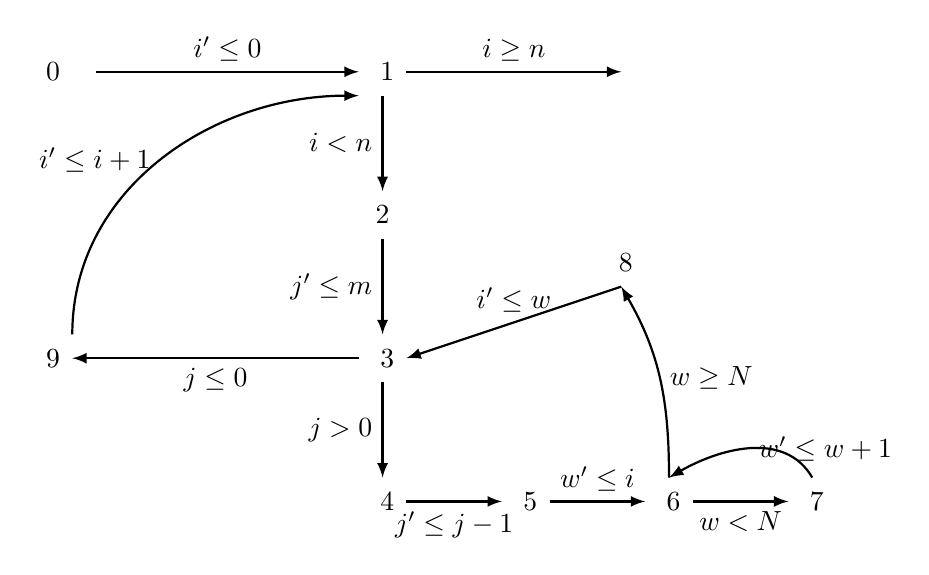
\begin{tikzpicture}[scale=\textwidth/20cm,samples=200]
\draw[] (-7, 10) circle (0pt) node{{ $0$}};
\draw[] (0, 10) circle (0pt) node{{ $1$}};
\draw[] (6, 10) circle (0pt) node {{$\lex$}};
\draw[] (0, 7) circle (0pt) node{{$2$}};
\draw[] (0, 4) circle (0pt) node{{ $3$}};
\draw[] (-7, 4) circle (0pt) node{{ $9$}};
\draw[] (0, 1) circle (0pt) node{{ $4$}};
\draw[] (3, 1) circle (0pt) node{{ $5$}};
\draw[] (6, 1) circle (0pt) node{{ $6$}};
\draw[] (9, 1) circle (0pt) node{{ $7$}};
\draw[] (5, 6) circle (0pt) node{{ $8$}};
% Counter Variables
%
% Control Flow Edges:
\draw[ thick, -latex] (-6, 10)  -- node [above] {$i' \leq 0$}(-0.5, 10);
\draw[ thick, -latex] (0, 9.5)  -- node [left] {$i < n$} (0, 7.5) ;
\draw[ thick, -latex] (0, 6.5)  -- node [left] {$j' \leq m$} (0, 4.5) ;
\draw[ thick, -latex] (0, 3.5)  -- node [left] {$j > 0$} (0, 1.5) ;
\draw[ thick, -latex] (-0.5, 4)  -- node [below] {$j \leq 0$} (-6.5, 4) ;
\draw[ thick, -latex] (-6.5, 4.5)  to  [out=90,in=180]  node [left] {$i' \leq i + 1$ }(-0.5, 9.5);
\draw[ thick, -latex] (0.5, 10)  -- node [above] {$i \geq n$}  (5, 10);
\draw[ thick, -latex] (0.5, 1)  -- node [below] {$j' \leq j - 1$}  (2.5, 1);
\draw[ thick, -latex] (3.5, 1)  -- node [above] {$w' \leq i$}  (5.5, 1);
\draw[ thick, -latex] (6.5, 1)  -- node [below] {$w < N$}  (8.5, 1);
\draw[ thick, -latex] (6, 1.5)  to [out=90,in=-60] node [right] {$w \geq N$}  (5, 5.5);
\draw[ thick, -latex] (9, 1.5)  to  [out=120,in=30] node [right] {$w' \leq w + 1$}  (6, 1.5);
\draw[ thick, -latex] (5, 5.5)  to  node [above] {$i' \leq w$ }(0.5, 4);
\end{tikzpicture}
\caption{}
  \end{centering}
  \end{subfigure}
\caption{
(a) The Example of Nested Loop with Related Iterators
  (b) The Abstract Execution Control Flow Graph}
    \label{fig:threeNestedWhile}
\end{figure}
}
\end{example}

\begin{enumerate}
  \item  \textbf{The Abstract Control Flow Graph}: Figure~\ref{fig:threeNestedWhile}(b).

  \item \textbf{Program Refinement}
  \\
  {Simple Transition Paths:}
  %  are computed as follows,
  \\
$
      \begin{array}{llll}
          \tpath_0 = (0 \to 1)
          &
          \tpath_1 = (1 \to 2 \to 3)
          &           
          \tpath_2 = (3 \to 4 \to 5 \to 6)
          &
          \tpath_3 = (6 \to 7 \to 6)
          \\
          \tpath_6 = (1 \to \lex)
          &
          \tpath_4 = (6 \to 8 \to 3)
          &
          \tpath_5 = (3 \to 9 \to 1)
      \end{array}
$
  \\
  Refined Program:
\\
$
  \rprog = \tpath_0 ; 
1: \rprepeat(\tpath_1; 3: \rprepeat(\tpath_2; 6: \rprepeat(\tpath_3); \tpath_4); \tpath_5); \tpath_6
$
\\
Let $\rprog_1 = \rprepeat(\tpath_1; 3: \rprepeat(\tpath_2; 6: \rprepeat(\tpath_3); \tpath_4); \tpath_5)$
\\
$\rprog_3 = \rprepeat(\tpath_2; 6: \rprepeat(\tpath_3); \tpath_4)$
\\
$\rprog_6 = \rprepeat(\tpath_3)$
  \item {Path Local Reachability-bound}:
\\
$\outinB(1: \rprog_1, \tpath_1) = n - N$ \quad
$\outinB(1: \rprog_1, \tpath_5) = n - N$ \quad
$\outinB(3: \rprog_3, \tpath_2) = m$ \\
$\outinB(3: \rprog_3, \tpath_4) = m$ \quad
$\outinB(6: \rprog_6, \tpath_3) = N$ \quad
%
\\
Loop Bounds:
\\
$BD(\tpath_0) = 1$
\quad
$BD(\tpath_6) = 1$
\quad
$BD( \rprepeat(\tpath_3)) = N $
\quad
$BD(\rprog_3) = m $
\quad
$BD(\rprog_1) = n - N $
%
\item Loop Reachability-bound:
\\
\highlight{
$\lpchB(1: \rprog_1, \tpath_1) = n - N$ \quad
$\lpchB(1: \rprog_1, \tpath_5) = n - N$ \quad
$\lpchB(1: \rprog_1, \tpath_2) = n$ \\ 
$\lpchB(1: \rprog_1, \tpath_4) = n$ \quad
$\lpchB(1: \rprog_1, \tpath_3) = 1$ \quad
$\lpchB(3: \rprog_3, \tpath_4) = m$ \\
$\lpchB(3: \rprog_3, \tpath_2) = m$ \quad
$\lpchB(3: \rprog_3, \tpath_3) = 1$ \quad 
$\lpchB(6: \rprog_6, \tpath_3) = N$
}
%
%
\item Path Global Reachability-bound:
\\
$\inoutB(\rprog, \tpath_1) = n - N$ \quad
$\inoutB(\rprog, \tpath_2) = n \times m$ \quad
$\inoutB(\rprog, \tpath_0) = 1$ 
\quad
$\inoutB(\rprog, \tpath_5) = n - N$ \quad
$\inoutB(\rprog, \tpath_4) = n \times m$ \quad
$\inoutB(\rprog, \tpath_6) = 1$ 
\quad
$\inoutB(\rprog, \tpath_3) = N$
%
\item The Reachability-bound:
\\
$\psRB(0) = \psRB(\lex) = 1$ \quad
$\psRB(1) = n - N + 1$ \quad
$\psRB(2) = \psRB(9) = n - N$ \quad
$\psRB(7) = N$
\\
$\psRB(3) = n - N + n \times m$ \quad
$\psRB(4) = \psRB(5) = \psRB(8) = n \times m$ \quad
$\psRB(6) = N + n \times m$ 
\end{enumerate}
